    
    
    

    
    \hypertarget{bisection-method-for-finding-root}{%
\section{Bisection method for finding
root}\label{bisection-method-for-finding-root}}

    Bisection method is a root-finding algorithm that could be used to find
any one root of a continuous function \(f(x)\), which could be evaluated
at two points \(a\) and \(b\) such that, \[f(a) \cdot f(b) < 0\]

\begin{figure}
\centering
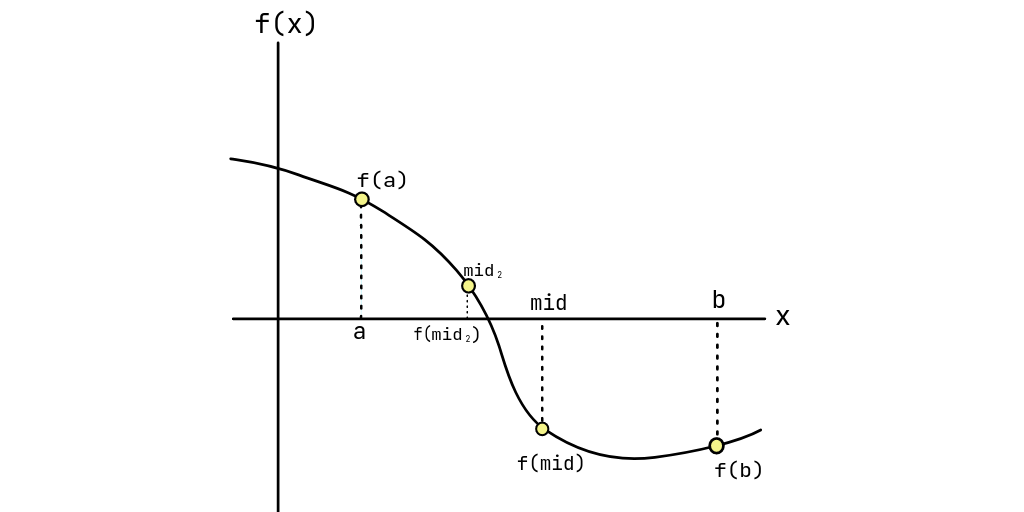
\includegraphics{resources/bisection-1.png}
\caption{resources/bisection-1.png}
\end{figure}

For the Bisection method to work we would have to provide the function
\(f(x)\) along with two points \(a\) and \(b\) for which the function
will yeild two values, \(f(a)\) and \(f(b)\) of opposite signs. Then the
Bisection method works by bisecting the inteval \(a\) and \(b\), and
using the midpoint, say \(mid = \frac{a + b}{2}\), as a guess for the
root.

If the guessed root isn't close enough to zero, then there are two
possibilities, \[f(a) \cdot f(mid) < 0\] \[f(b) \cdot f(mid) < 0\]

For the first case \(b\) shall be shifted to the \(mid\), and for the
later \(a\) shall be shifted at the \(mid\).

\begin{align}
    & b = mid, & if \; & f(a) \cdot f(mid) < 0 \\
    & a = mid, & if \; & f(b) \cdot f(mid) < 0
\end{align}

Now the next guess would be the midpoint between the updated \(a\) and
\(b\). This method is to be repeated until a suitable enough guess for
the root close to zero has been found.

    \hypertarget{code}{%
\subsection{Code}\label{code}}

    \begin{tcolorbox}[breakable, size=fbox, boxrule=1pt, pad at break*=1mm,colback=cellbackground, colframe=cellborder]
\prompt{In}{incolor}{1}{\boxspacing}
\begin{Verbatim}[commandchars=\\\{\}]
\PY{k+kn}{from} \PY{n+nn}{numpy} \PY{k+kn}{import} \PY{n}{e}
\end{Verbatim}
\end{tcolorbox}

    \begin{tcolorbox}[breakable, size=fbox, boxrule=1pt, pad at break*=1mm,colback=cellbackground, colframe=cellborder]
\prompt{In}{incolor}{2}{\boxspacing}
\begin{Verbatim}[commandchars=\\\{\}]
\PY{c+c1}{\PYZsh{} Code for finding root using Bisection method}
\PY{k}{def} \PY{n+nf}{find\PYZus{}root\PYZus{}bisection}\PY{p}{(}\PY{n}{f}\PY{p}{,} \PY{n}{a}\PY{p}{,} \PY{n}{b}\PY{p}{,} \PY{n}{tolerance}\PY{o}{=}\PY{l+m+mf}{0.001}\PY{p}{)}\PY{p}{:}

    \PY{c+c1}{\PYZsh{} Checking if it is possible to find the root using Bisection method}
    \PY{k}{if} \PY{n}{f}\PY{p}{(}\PY{n}{a}\PY{p}{)} \PY{o}{*} \PY{n}{f}\PY{p}{(}\PY{n}{b}\PY{p}{)} \PY{o}{\PYZgt{}}\PY{o}{=} \PY{l+m+mi}{0}\PY{p}{:}
        \PY{k}{raise} \PY{n+ne}{ValueError}\PY{p}{(}\PY{l+s+s2}{\PYZdq{}}\PY{l+s+s2}{f(a)*f(b) must be less than zero.}\PY{l+s+s2}{\PYZdq{}}\PY{p}{)}

    \PY{c+c1}{\PYZsh{} Evaluating the root}
    \PY{k}{while} \PY{n+nb}{abs}\PY{p}{(}\PY{n}{a} \PY{o}{\PYZhy{}} \PY{n}{b}\PY{p}{)} \PY{o}{\PYZgt{}} \PY{n}{tolerance}\PY{p}{:}

        \PY{c+c1}{\PYZsh{} Evaluating the midpoint}
        \PY{n}{mid} \PY{o}{=} \PY{p}{(}\PY{n}{a} \PY{o}{+} \PY{n}{b}\PY{p}{)} \PY{o}{/} \PY{l+m+mi}{2}

        \PY{c+c1}{\PYZsh{} Updating `a` and `b` as required}
        \PY{k}{if} \PY{n}{f}\PY{p}{(}\PY{n}{a}\PY{p}{)} \PY{o}{*} \PY{n}{f}\PY{p}{(}\PY{n}{mid}\PY{p}{)} \PY{o}{\PYZlt{}} \PY{l+m+mi}{0}\PY{p}{:}
            \PY{n}{b} \PY{o}{=} \PY{n}{mid}
        \PY{k}{elif} \PY{n}{f}\PY{p}{(}\PY{n}{b}\PY{p}{)} \PY{o}{*} \PY{n}{f}\PY{p}{(}\PY{n}{mid}\PY{p}{)} \PY{o}{\PYZlt{}} \PY{l+m+mi}{0}\PY{p}{:}
            \PY{n}{a} \PY{o}{=} \PY{n}{mid}

    \PY{k}{return} \PY{n}{mid}
\end{Verbatim}
\end{tcolorbox}

    \hypertarget{examples}{%
\subsection{Examples}\label{examples}}

    \hypertarget{x2-2}{%
\subsubsection{\texorpdfstring{\[x^2 = 2\]}{x\^{}2 = 2}}\label{x2-2}}

\[f(x) = x^2 - 2\]

    \begin{tcolorbox}[breakable, size=fbox, boxrule=1pt, pad at break*=1mm,colback=cellbackground, colframe=cellborder]
\prompt{In}{incolor}{3}{\boxspacing}
\begin{Verbatim}[commandchars=\\\{\}]
\PY{k}{def} \PY{n+nf}{f}\PY{p}{(}\PY{n}{x}\PY{p}{)}\PY{p}{:}
    \PY{k}{return} \PY{n}{x}\PY{o}{*}\PY{o}{*}\PY{l+m+mi}{2} \PY{o}{\PYZhy{}} \PY{l+m+mi}{2}


\PY{n}{a} \PY{o}{=} \PY{l+m+mi}{1}
\PY{n}{b} \PY{o}{=} \PY{l+m+mi}{5}

\PY{n}{find\PYZus{}root\PYZus{}bisection}\PY{p}{(}\PY{n}{f}\PY{p}{,} \PY{n}{a}\PY{p}{,} \PY{n}{b}\PY{p}{)}
\end{Verbatim}
\end{tcolorbox}

            \begin{tcolorbox}[breakable, size=fbox, boxrule=.5pt, pad at break*=1mm, opacityfill=0]
\prompt{Out}{outcolor}{3}{\boxspacing}
\begin{Verbatim}[commandchars=\\\{\}]
1.4150390625
\end{Verbatim}
\end{tcolorbox}
        
    \hypertarget{x3---x2-x-e}{%
\subsubsection{\texorpdfstring{\[x^3 - x^2 + x = e\]}{x\^{}3 - x\^{}2 + x = e}}\label{x3---x2-x-e}}

\[f(x) = x^3 - x^2 + x - e\]

    \begin{tcolorbox}[breakable, size=fbox, boxrule=1pt, pad at break*=1mm,colback=cellbackground, colframe=cellborder]
\prompt{In}{incolor}{4}{\boxspacing}
\begin{Verbatim}[commandchars=\\\{\}]
\PY{k}{def} \PY{n+nf}{f}\PY{p}{(}\PY{n}{x}\PY{p}{)}\PY{p}{:}
    \PY{k}{return} \PY{n}{x}\PY{o}{*}\PY{o}{*}\PY{l+m+mi}{3} \PY{o}{\PYZhy{}} \PY{n}{x}\PY{o}{*}\PY{o}{*}\PY{l+m+mi}{2} \PY{o}{+} \PY{n}{x} \PY{o}{\PYZhy{}} \PY{n}{e}


\PY{n}{a} \PY{o}{=} \PY{l+m+mi}{0}
\PY{n}{b} \PY{o}{=} \PY{l+m+mi}{3}

\PY{n}{find\PYZus{}root\PYZus{}bisection}\PY{p}{(}\PY{n}{f}\PY{p}{,} \PY{n}{a}\PY{p}{,} \PY{n}{b}\PY{p}{)}
\end{Verbatim}
\end{tcolorbox}

            \begin{tcolorbox}[breakable, size=fbox, boxrule=.5pt, pad at break*=1mm, opacityfill=0]
\prompt{Out}{outcolor}{4}{\boxspacing}
\begin{Verbatim}[commandchars=\\\{\}]
1.519775390625
\end{Verbatim}
\end{tcolorbox}
        

    % Add a bibliography block to the postdoc
    
    
    
